\documentclass{standalone}
\usepackage{tikz}
\usetikzlibrary{matrix,scopes,arrows}
\tikzset{
  > = angle 60,
  mymx/.style={
    matrix of nodes,
    nodes=mynode,
    row sep=1.5em,
    column sep=1.5em,
    row 2/.style={nodes=rnd},
    row 1 column 2/.style={yshift=-1em},
    row 3 column 2/.style={yshift=1em},
  },
  mynode/.style={
    draw,
    text width=6em,
    align=center
  },
  rnd/.style={
    mynode,
    rounded corners=1.5ex
  }
}

\begin{document}
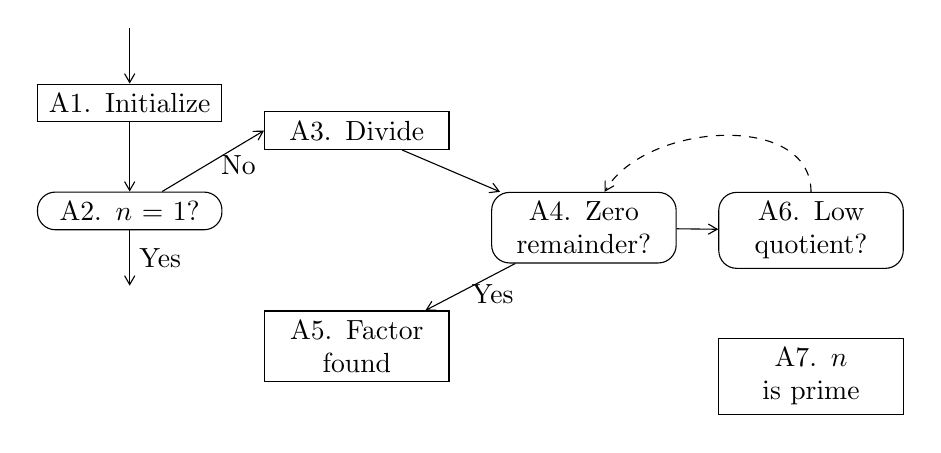
\begin{tikzpicture}
\matrix (mx) [mymx] {
  A1. Initialize & A3. Divide\\
  A2. $n=1$?     &                  & A4. Zero remainder? & A6. Low quotient?\\
                 & A5. Factor found &                     & A7. $n$ is prime\\
};
{[every edge/.style={draw,->}]
\draw ([yshift=2em]mx-1-1.north) edge (mx-1-1)
  (mx-1-1) edge (mx-2-1)
  (mx-2-1) edge node[midway,right] {Yes} ([yshift=-2em]mx-2-1.south)
  (mx-2-1) edge node[near end,below] {No}  (mx-1-2.west)
  (mx-1-2) edge (mx-2-3)
  (mx-2-3) edge node[near start,below] {Yes} (mx-3-2)
           edge (mx-2-4)
  ;
\draw[->, dashed] (mx-2-4) edge[out=90, in=60] (mx-2-3);
}
\end{tikzpicture}
\end{document}